\documentclass{sigchi-ext}
% Please be sure that you have the dependencies (i.e., additional
% LaTeX packages) to compile this example.
\usepackage[T1]{fontenc}
\usepackage{textcomp}
\usepackage[scaled=.92]{helvet} % for proper fonts
\usepackage{graphicx} % for EPS use the graphics package instead
\usepackage{balance}  % for useful for balancing the last columns
\usepackage{booktabs} % for pretty table rules
\usepackage{ccicons}  % for Creative Commons citation icons
\usepackage{ragged2e} % for tighter hyphenation
\usepackage{threeparttable}
\usepackage{rotating}
\usepackage{multirow}
% Some optional stuff you might like/need.
% \usepackage{marginnote}
% \usepackage[shortlabels]{enumitem}
% \usepackage{paralist}
% \usepackage[utf8]{inputenc} % for a UTF8 editor only

%% EXAMPLE BEGIN -- HOW TO OVERRIDE THE DEFAULT COPYRIGHT STRIP --
% \copyrightinfo{Permission to make digital or hard copies of all or
% part of this work for personal or classroom use is granted without
% fee provided that copies are not made or distributed for profit or
% commercial advantage and that copies bear this notice and the full
% citation on the first page. Copyrights for components of this work
% owned by others than ACM must be honored. Abstracting with credit is
% permitted. To copy otherwise, or republish, to post on servers or to
% redistribute to lists, requires prior specific permission and/or a
% fee. Request permissions from permissions@acm.org.\\
% {\emph{CHI'14}}, April 26--May 1, 2014, Toronto, Canada. \\
% Copyright \copyright~2014 ACM ISBN/14/04...\$15.00. \\
% DOI string from ACM form confirmation}
%% EXAMPLE END

% Paper metadata (use plain text, for PDF inclusion and later
% re-using, if desired).  Use \emtpyauthor when submitting for review
% so you remain anonymous.
\def\plaintitle{\sysname: Bicycle Behavior Tracking via Smartphones} 
\def\plainkeywords{Authors' choice; of terms; separated; by
  semicolons; include commas, within terms only; required.}
\def\plaingeneralterms{Documentation, Standardization}
\def\sysname{BeTracker }
\def\ie{i.e., }
\def\eg{e.g., }

\title{\plaintitle}

\numberofauthors{6}
% Notice how author names are alternately typesetted to appear ordered
% in 2-column format; i.e., the first 4 autors on the first column and
% the other 4 auhors on the second column. Actually, it's up to you to
% strictly adhere to this author notation.
\author{%
  \alignauthor{%
    \textbf{Weixi Gu}\\
    \affaddr{Tsinghua-Berkeley Shenzhen Institute} \\
    \affaddr{Tsinghua University} \\
    \email{guweixigavin@gmail.com} }\alignauthor{%
    \textbf{Fifth Author}\\
    \affaddr{YetAuthorCo, Inc.}\\
    \affaddr{Authortown, BC V6M 22P Canada}\\
    \email{author5@anotherco.com} } \vfil \alignauthor{%
    \textbf{Zimu Zhou}\\
    \affaddr{ Computer Engineering and Networks Laboratory}\\
    \affaddr{ ETH Zurich}\\
    \email{zzhou@tik.ee.ethz.ch} }\alignauthor{%
    \textbf{Sixth Author}\\
    \affaddr{Universit\'e de Auteur-Sud}\\
    \affaddr{40222 Auteur France}\\
    \email{author6@author.fr} } \vfil \alignauthor{%
    \textbf{}\\
    \affaddr{ }\\
    \affaddr{ }\\
    \email{} \\ }\alignauthor{%
    \textbf{Seventh Author}\\
    \affaddr{Department of Skrywer}\\
    \affaddr{University of Umbhali}\\
    \affaddr{Cape Town, South Africa}\\
    \email{author7@umbhaliu.ac.za} } }

% Make sure hyperref comes last of your loaded packages, to give it a
% fighting chance of not being over-written, since its job is to
% redefine many LaTeX commands.
\definecolor{linkColor}{RGB}{6,125,233}
\hypersetup{%
	pdftitle={\plaintitle},
	%  pdfauthor={\plainauthor},
	pdfauthor={\emptyauthor},
	pdfkeywords={\plainkeywords},
	bookmarksnumbered,
	pdfstartview={FitH},
	colorlinks,
	citecolor=black,
	filecolor=black,
	linkcolor=black,
	urlcolor=linkColor,
	breaklinks=true,
}
% \reversemarginpar%

\begin{document}

%% For the camera ready, use the commands provided by the ACM in the Permission Release Form.
%\CopyrightYear{2007}
%\setcopyright{rightsretained}
%\conferenceinfo{WOODSTOCK}{'97 El Paso, Texas USA}
%\isbn{0-12345-67-8/90/01}
%\doi{http://dx.doi.org/10.1145/2858036.2858119}
%% Then override the default copyright message with the \acmcopyright command.
%\copyrightinfo{\acmcopyright}
\maketitle

% Uncomment to disable hyphenation (not recommended)
% https://twitter.com/anjirokhan/status/546046683331973120
\RaggedRight{}

% Do not change the page size or page settings.
\begin{abstract}
Monitoring the bicycle safety is of great importance. The current methods either require specific hardware supports or are expensive. In this paper, we propose \sysname, a smartphone-based system to track bicyclist movements and alarm their dangerous riding behaviors in real time. Preliminary experiments over 15 days show that the overall detection accuracy of \sysname on riding behavior achieves 94.6\%,  satisfying the practical operation in daily usage.                   
\end{abstract}
%
\keywords{\plainkeywords}

\category{H.5.m}{Information interfaces and presentation (e.g.,
  HCI)}{Miscellaneous}\category{See}{\url{http://acm.org/about/class/1998/}}{for
  full list of ACM classifiers. This section is required.}
%
\section{Introduction}
% study problem
Bicycle is a worldwide and principal transportation tool due to its efficiency, environment-friendly and cheap. However, the bicycle safety is easily overlooked by many cyclists. According to the recent report, there were 726 cyclists killed and an additional 50,000 injured in motor vehicle traffic crashes in 2014 \cite{bib:Bic2014}.
Dangerous riding behaviors is one of a main factor of this kind of accident. 
Specifically, the frequent lane weaving or stand riding is easy for the bike rider to loss balance, and riding a bike against the direction of legal traffic usually causes head-on collision or traffic congestion. 
Therefore, a real-time, ubiquitous and efficient system to monitor the bicyclist behavior is of great importance. 
% what is related work

Improving the bicycle safety is a key issue in human lifetime, and it has been studied by a broad-range of research works. Cyber-Physical bicycle \cite{Bib:imp2010} performs automated rear-approaching vehicle detection via video and audio sensors. LightLane \cite{bib:Lig2014} highlights a bike path around a bicycle on the roadway by projecting an image, reminding the motorists to keep a safe passing distance. However, these works require professional hardware supports.  BikeNet \cite{Bib:Bik2009} constructs a mobile sensing platform on a bicycle to gather the riding data and the environmental data. \sysname takes one step further of this work,  providing a pervasive and efficient system to monitor the bicyclist riding behaviors with smartphones. It evokes the embedded accelerometers and gyrometers of smartphones to monitor the cyclists' movements and employs the GPS to track their riding directions, which infers the two common and dangerous riding actions (\ie the frequent lane weaving and standing riding) and detects the wrong-way riding.  
Compared with previous works, \sysname gets rid of the professional hardware equipments, and provides an real-time alarm when the cyclists run in an illegal bike way. 

The key challenges are from two sides. 1) How to identify discriminative behaviors of the riders from noisy environmental data. 2) How to determine the legal riding directions of cycleways without knowledges.   
To copy with this issue, we design specific feature-extraction mechanism for each kind of data, and construct a crowdsourcing platform to learn the legal riding direction of cycleways. 
\sysname has been evaluated on eight users over two weeks. The experimental results show that the detection accuracy of three type of behaviors are all over XX\%, while its energy cost keeps below XX\% per hours, which is satisfied with the practical operation in daily life.  

\begin{figure}
  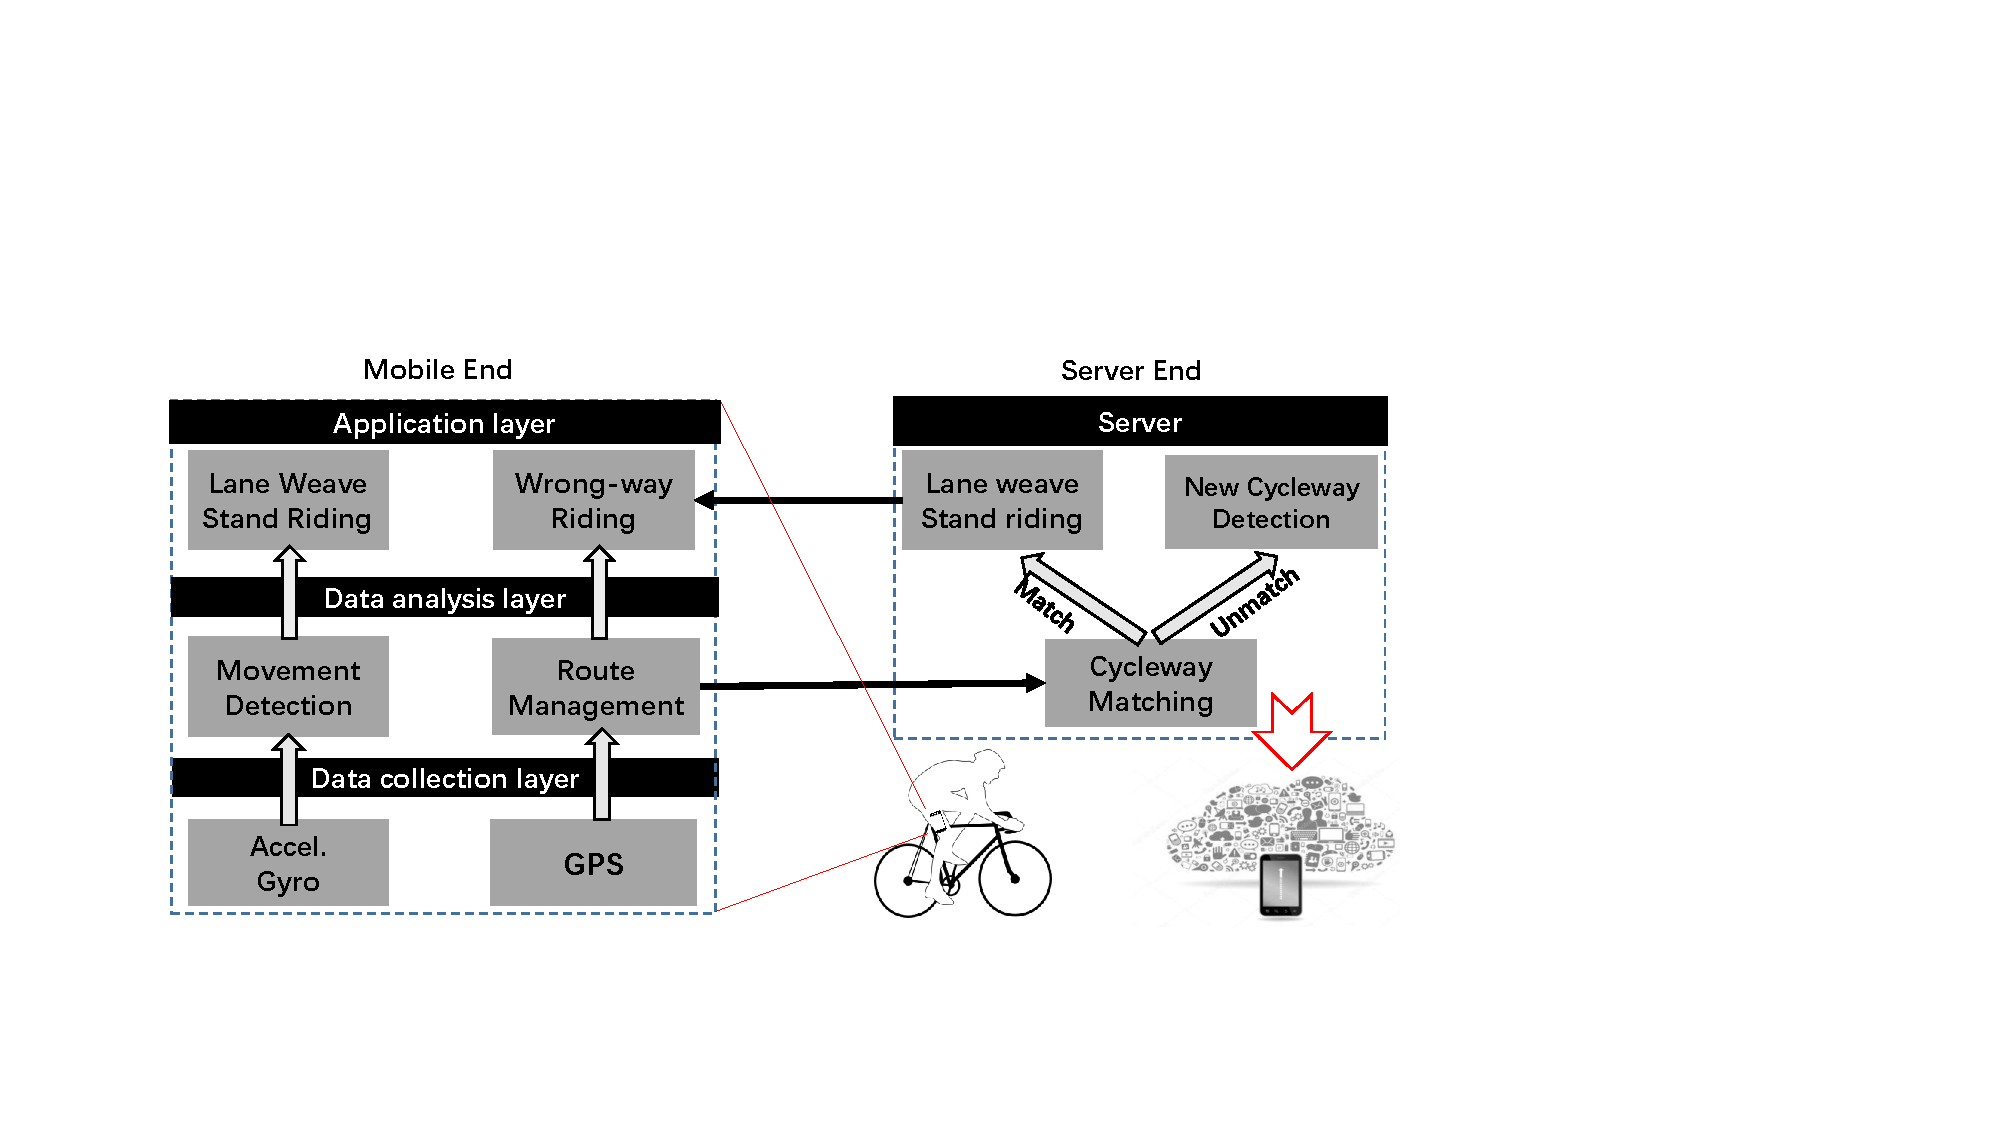
\includegraphics[width=0.9\columnwidth]{figures/sys.pdf}
  \caption{The system architecture.}~\label{fig:sys}
\end{figure}


%\begin{marginfigure}[1pc]
%  \begin{minipage}{\marginparwidth}
%    \centering
%    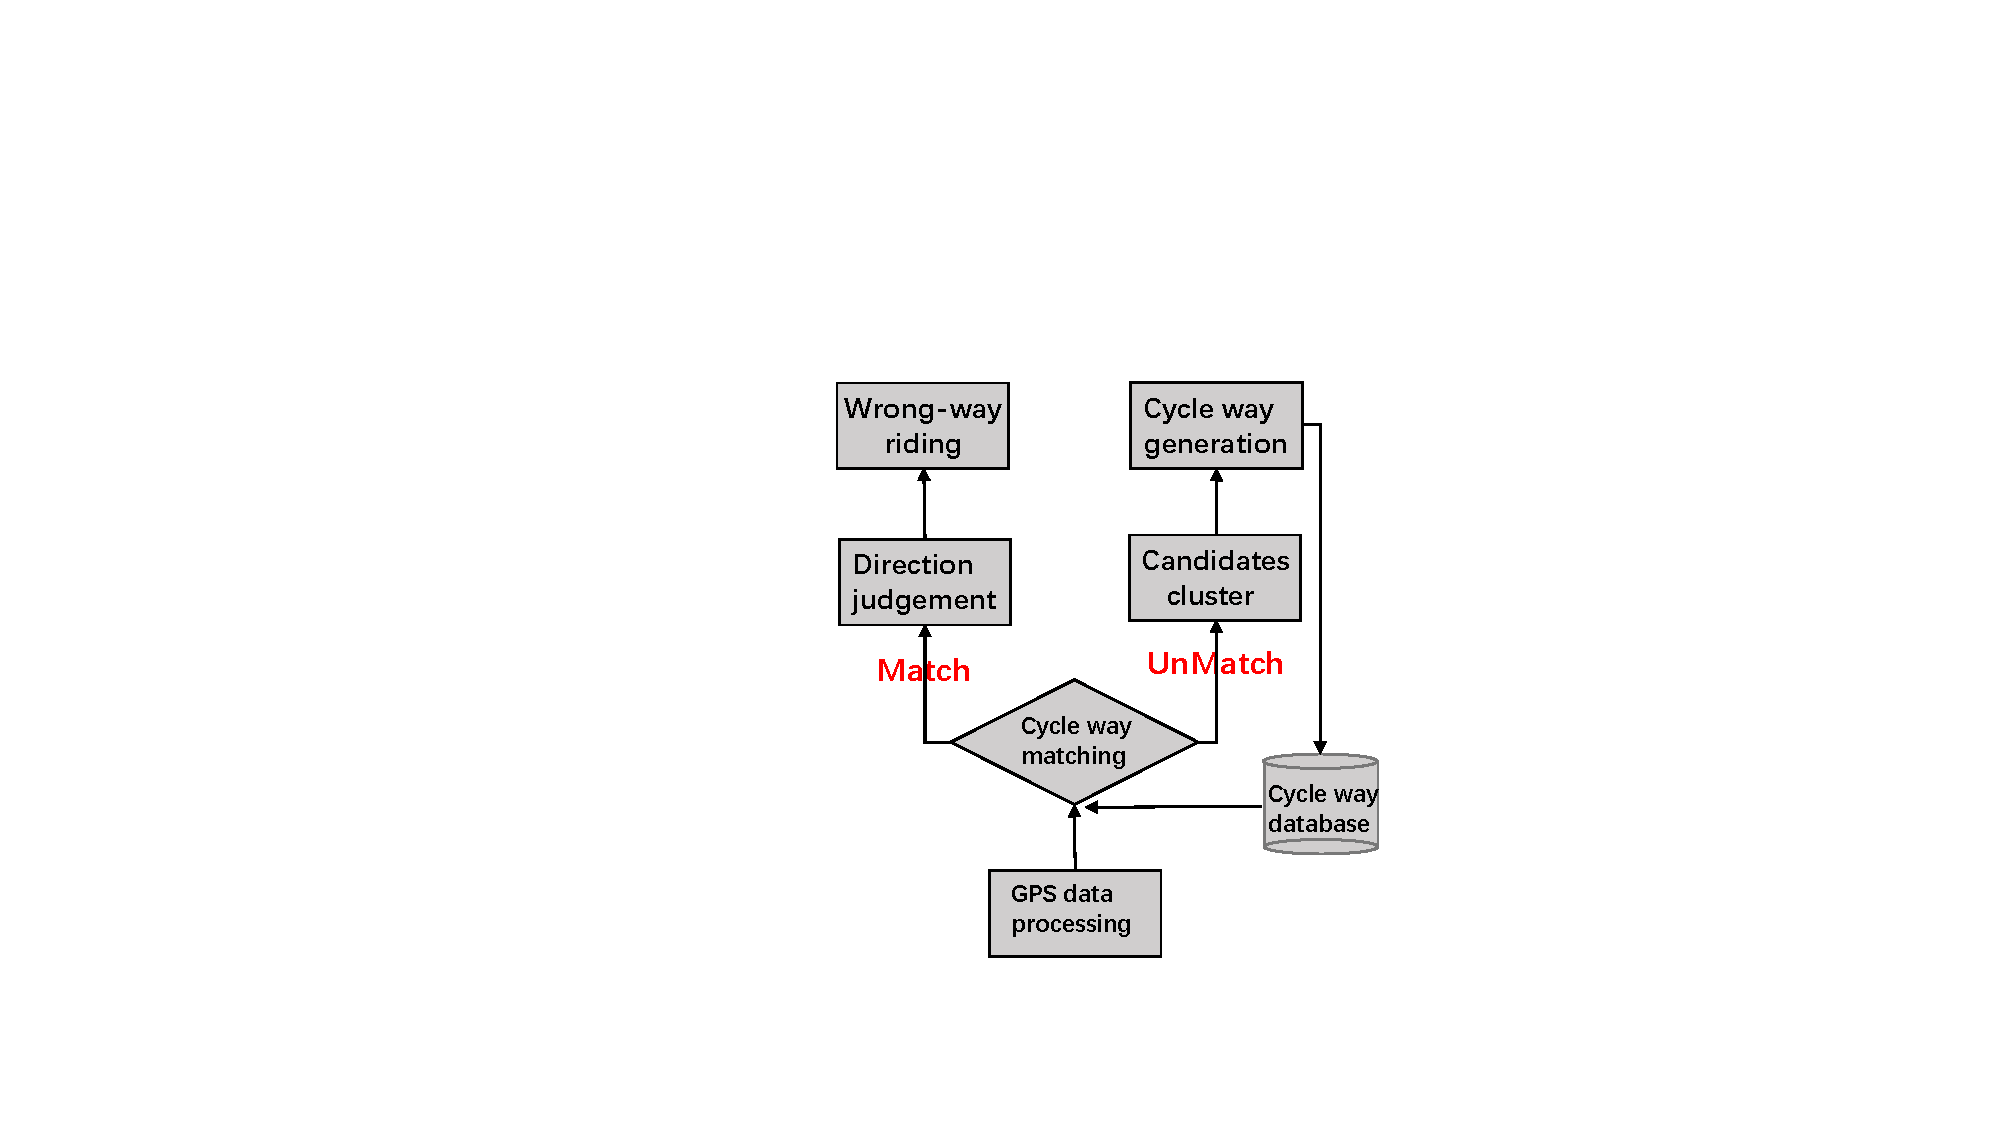
\includegraphics[width=0.9\marginparwidth]{figures/gps_workflow.pdf}
%    \caption{In ~\label{fig:marginfig}
%  \end{minipage}
%\end{marginfigure}


\section{ System Overview}
As shown in Fig. \ref{fig:sys}, \sysname is composed of the mobile end and the server end.  In mobile end, \sysname employs sensors of smartphones to collect the sensory data from bicyclists' physical movements and their traffic geographic GPS information at \textbf{data collection layer}, and then processes them at \textbf{data analysis layer}. The movement detection and route results are uploaded to \textbf{the application layer}. Once dangerous events are detected, \sysname sends an alarms to remind the bicyclists. 
The design of \sysname architecture is specified as follows.

\section{System Design} 
\subparagraph{Data collection layer}
As the smartphone is worn with the riders while they are riding, the cyclists' behaviors can be recorded by the sensors of smartphones.  \sysname evokes the acceleration and angular acceleration to learn the bicyclists' behavior information. Meanwhile, \sysname leverages GPS of smartphone to record the riders' traffic routes for the riding directions learning. 
The two kinds of sensory data are uploaded to the data analysis layer for the riding event detection.
\subparagraph{Data analysis layer} 

\begin{table}[h]
	\centering
	\caption{Selected Features of Riding Bicycle}
	\label{feature_table}
	\begin{threeparttable}
		\begin{tabular}{|l|l|}
			\hline
			\textbf{Feature}               & \textbf{Expression} \\ \hline
			Average Magnitude              &      $\sum_{j=1}^{N}a_{j}$              \\ \hline
			Standard Deviation             &      $\sqrt{\frac{1}{N}\sum_{j=1}^{N}(a_{j}-\mu )}$  \\ \hline
			Average Absolute Difference    &      $\frac{1}{N}\sum_{j=1}^{N}\left |a_{j}-\mu   \right |$\\ \hline
			Average Resultant Acceleration &      $\frac{1}{N}\sum_{j=1}^{N}\left |a_{xj}^2+a_{yj}^2+a_{zj}^2 \right |$   \\  \hline
			Binned Distribution            &      $\sum_{i=1}^{K}\sum_{j=1}^{N}sign\left [a_{j}-a_{min}+\frac{(i-1)}{M}(a_{max}-a_{min})\right ]\left [a_{min}+\frac{i}{M}(a_{max}-a_{min}) -a_j \right ]$              \\ \hline
		\end{tabular}
		\begin{tablenotes}
			\footnotesize
			\item[1] $a_{xj}$, $a_{yj}$ and $a_{zj}$ are the $j$th sample of three axes of the accelerometer in the sliding window. $a_{j}$ is the average square root of $a_{xj}$, $a_{yj}$ and $a_{zj}$. $a_{max}$, $a_{min}$ and $\mu$ are the maximum, minimum and the average value in the sliding window.  $N$ is the length of the sliding window. 
		\end{tablenotes}
	\end{threeparttable}
\end{table}


Riding movement detection and riding route management are two function modules in this layer. 

In \textit{movement detection module}, \sysname divides the riding behavior by three events: 1) frequent Lane weaving: weaving or swaying across the lane more than two times/minute;  2) Stand riding: the rider standing on the pedal to ride and 3) Normal riding. 
Lane weaving and stand riding are regards as two dangerous cases when the cyclists are riding on the road, which easily result to the cyclists loss their balance.
Intuitively, the acceleration and angular acceleration traces are exhibited distinct patterns on the three kinds of riding actions. The frequent sways during the lane weaving amplitude the force of the left and right sides, and thus improve the magnitude of angular acceleration directly. For the standing riding, the movements of cyclist's legs are greater than those of standard riding, which result in the higher of acceleration magnitude.
The distinct acceleration patterns of the three movements in Fig. \ref{fig:acc} demonstrate this point. The amplitude of the angular acceleration of lane weaving and the acceleration of the standing riding  are significantly larger than those of standard riding.  Accordingly, \sysname enables to predict the three riding movements by the acceleration features in Table~\ref{feature_table}. Considering the temporal-dependent in the acceleration pattern, we adopted Hidden Markov Model (HMM) for events classification.
\begin{figure}[h]
	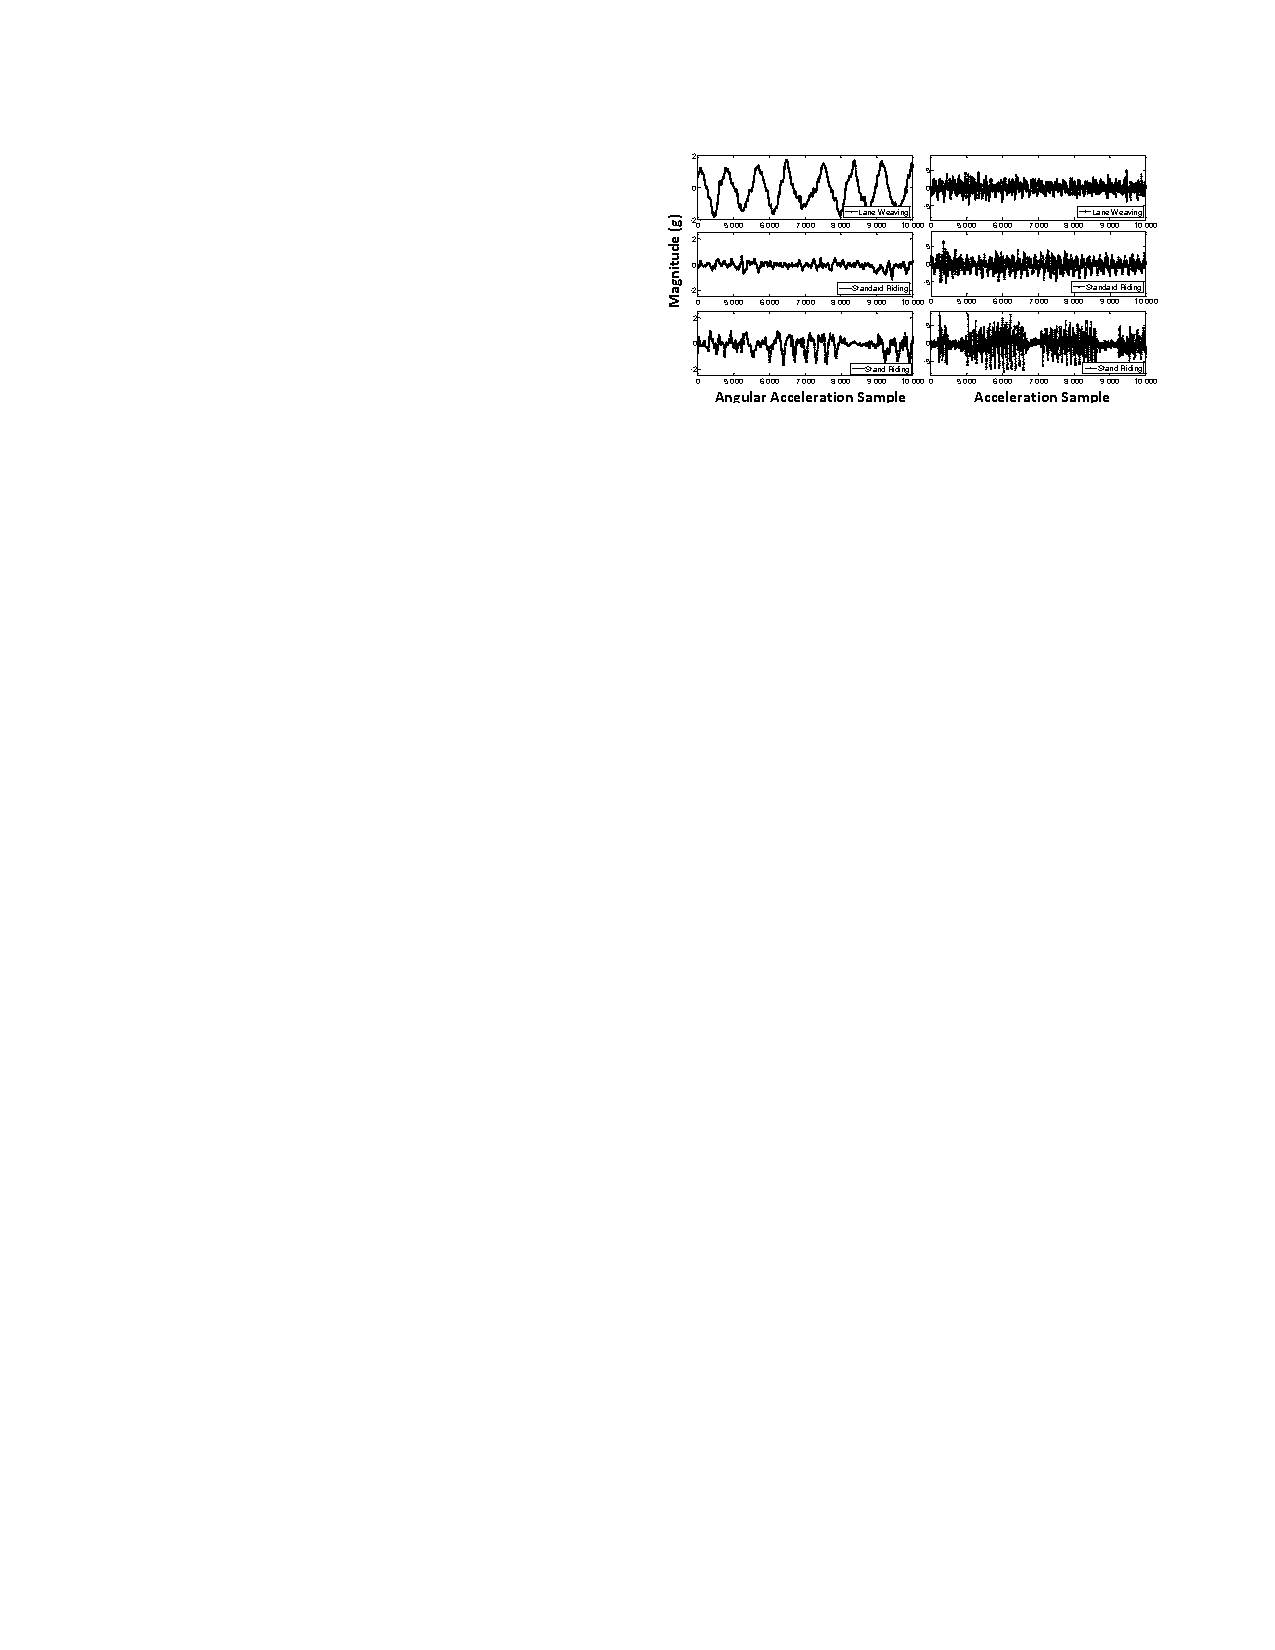
\includegraphics[width=0.9\columnwidth]{figures/acc.pdf}
	\caption{The angular acceleration and acceleration samples.}~\label{fig:acc}
\end{figure}

In \textit{wrong-way riding detection module}, \sysname aims to detect whether the user rides against the legal directions of the route.
Fig.~\ref{fig:gps_workflow} illustrates the work flow of the wrong-way riding detection. 

\begin{figure}[h]
	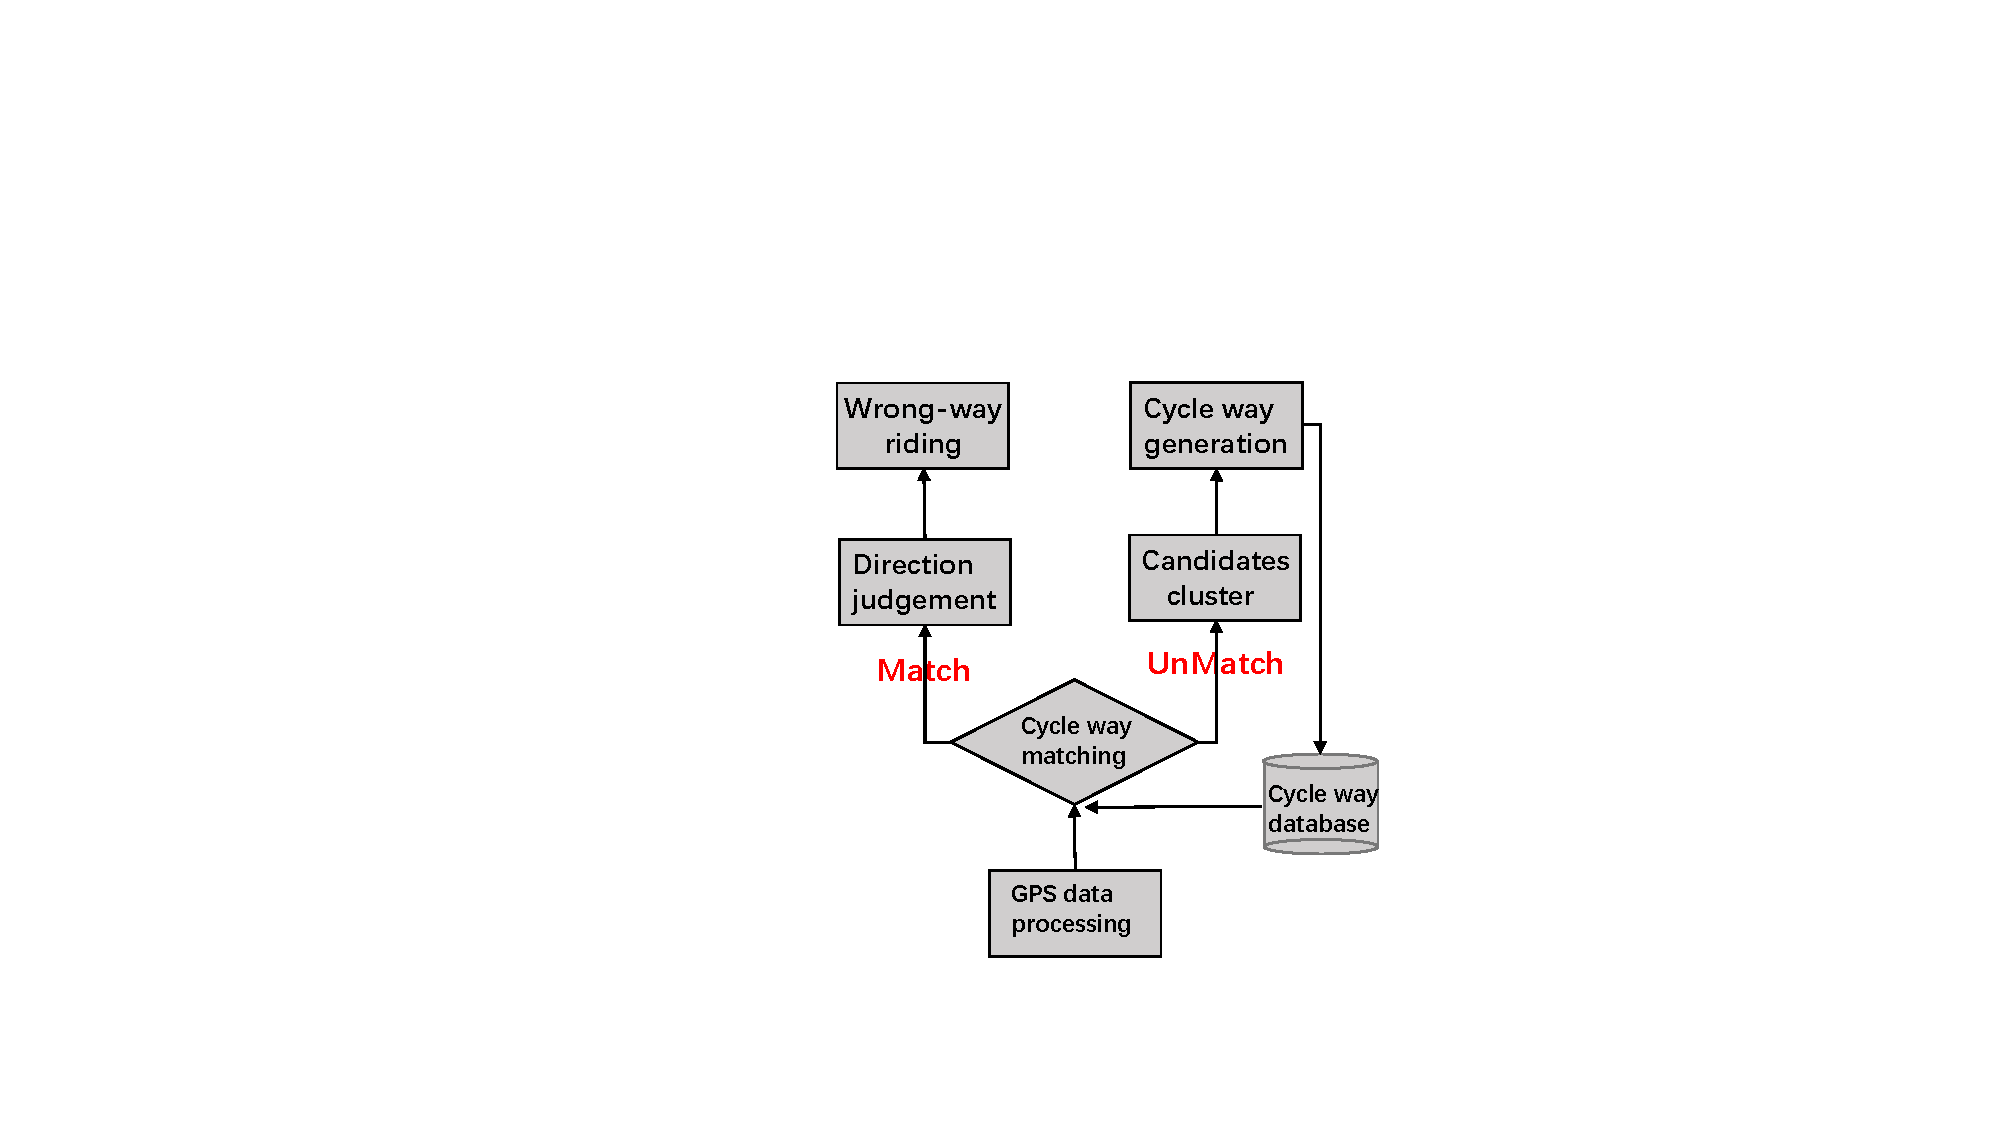
\includegraphics[width=0.7\columnwidth]{figures/gps_workflow.pdf}
	\caption{The angular acceleration and acceleration samples.}~\label{fig:gps_workflow}
\end{figure}
%
\sysname first conducts the GPS data process. Since GPS samples are easily influenced by the environment, \sysname eliminates its noise by removing the GPS samples whose error radius are larger than 20 meters, and adopts the Weighted Moving Average (WMA) to smooth the them.  Fig.~\ref{fig:gps_trace} illustrates the effects of noise elimination on the GPS traces

\begin{figure}[h]
	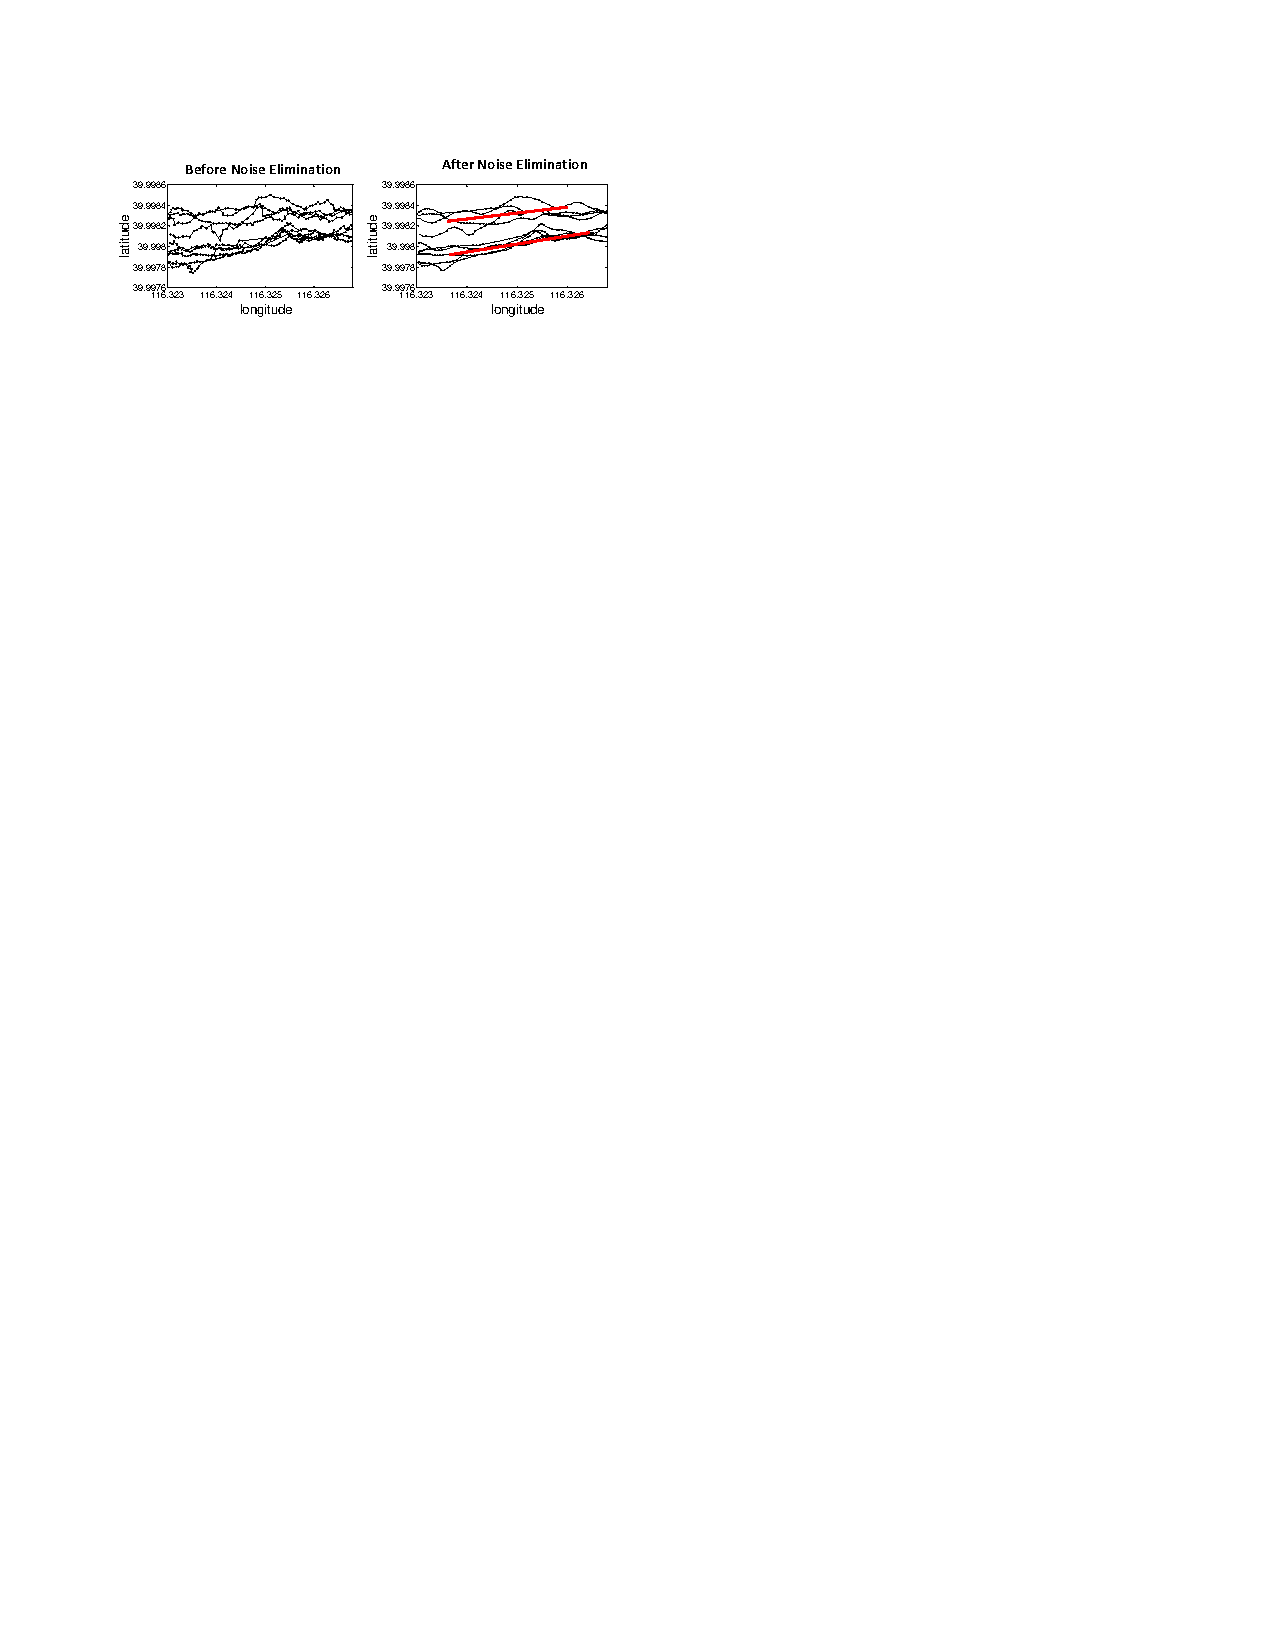
\includegraphics[width=0.9\columnwidth]{figures/GPS_trace.pdf}
	\caption{The GPS traces before and after noise elimination.}~\label{fig:gps_trace}
\end{figure}
%
Afterwards, \sysname delivers the GPS traces to the server and match it with the GPS trajectories in the server by Dynamic Time Warping (DTW). If matched, \sysname determines the cyclist's current position and then compares his/her riding direction with the legal direction of the cycleway.  \sysname computes a cyclist's riding direction by partitioning his GPS trajectory into disjointed segments. Assuming a GPS segment with a start co-ordinate ($X_{1}$, $Y_{1}$) and a end co-ordinate ($X_{2}$, $Y_{2}$), the riding direction $\tau$ of the cyclist is computed as $\tau=arctan(\frac{Y_{2}-Y_{1}}{X_{2}-X_{1}})$
If unmatched, \sysname regards this GPS trace as a new route candidates in the database. A new route is generated after more than there are three route candidates with less distance than preset threshold. A cycleway is calculated as the centerline of these candidates, and its legal distance is also consistent with the three candidate routes, which is calculated as above.  
%

\subparagraph{Application layer}
The application layer reminds the users of their dangerous riding events from the data analysis layer. When the dangerous events or circumstances detected by the system, \sysname delivers vibration and sound to remind users, and thus reduce the occurrence of the accidents. 

\section{Preliminary Evaluation}
We test \sysname from the performance of the riding events detection and the performance of the energy consumption. A total of 12 volunteers participants in our experiments, and each of them wears the smartphones on their trousers while they are riding according to our requirement. We manually label their behaviors. Fig.~\ref{fig:experiment_riding} illustrates the experiment scenarios. 

\begin{figure}[h]
	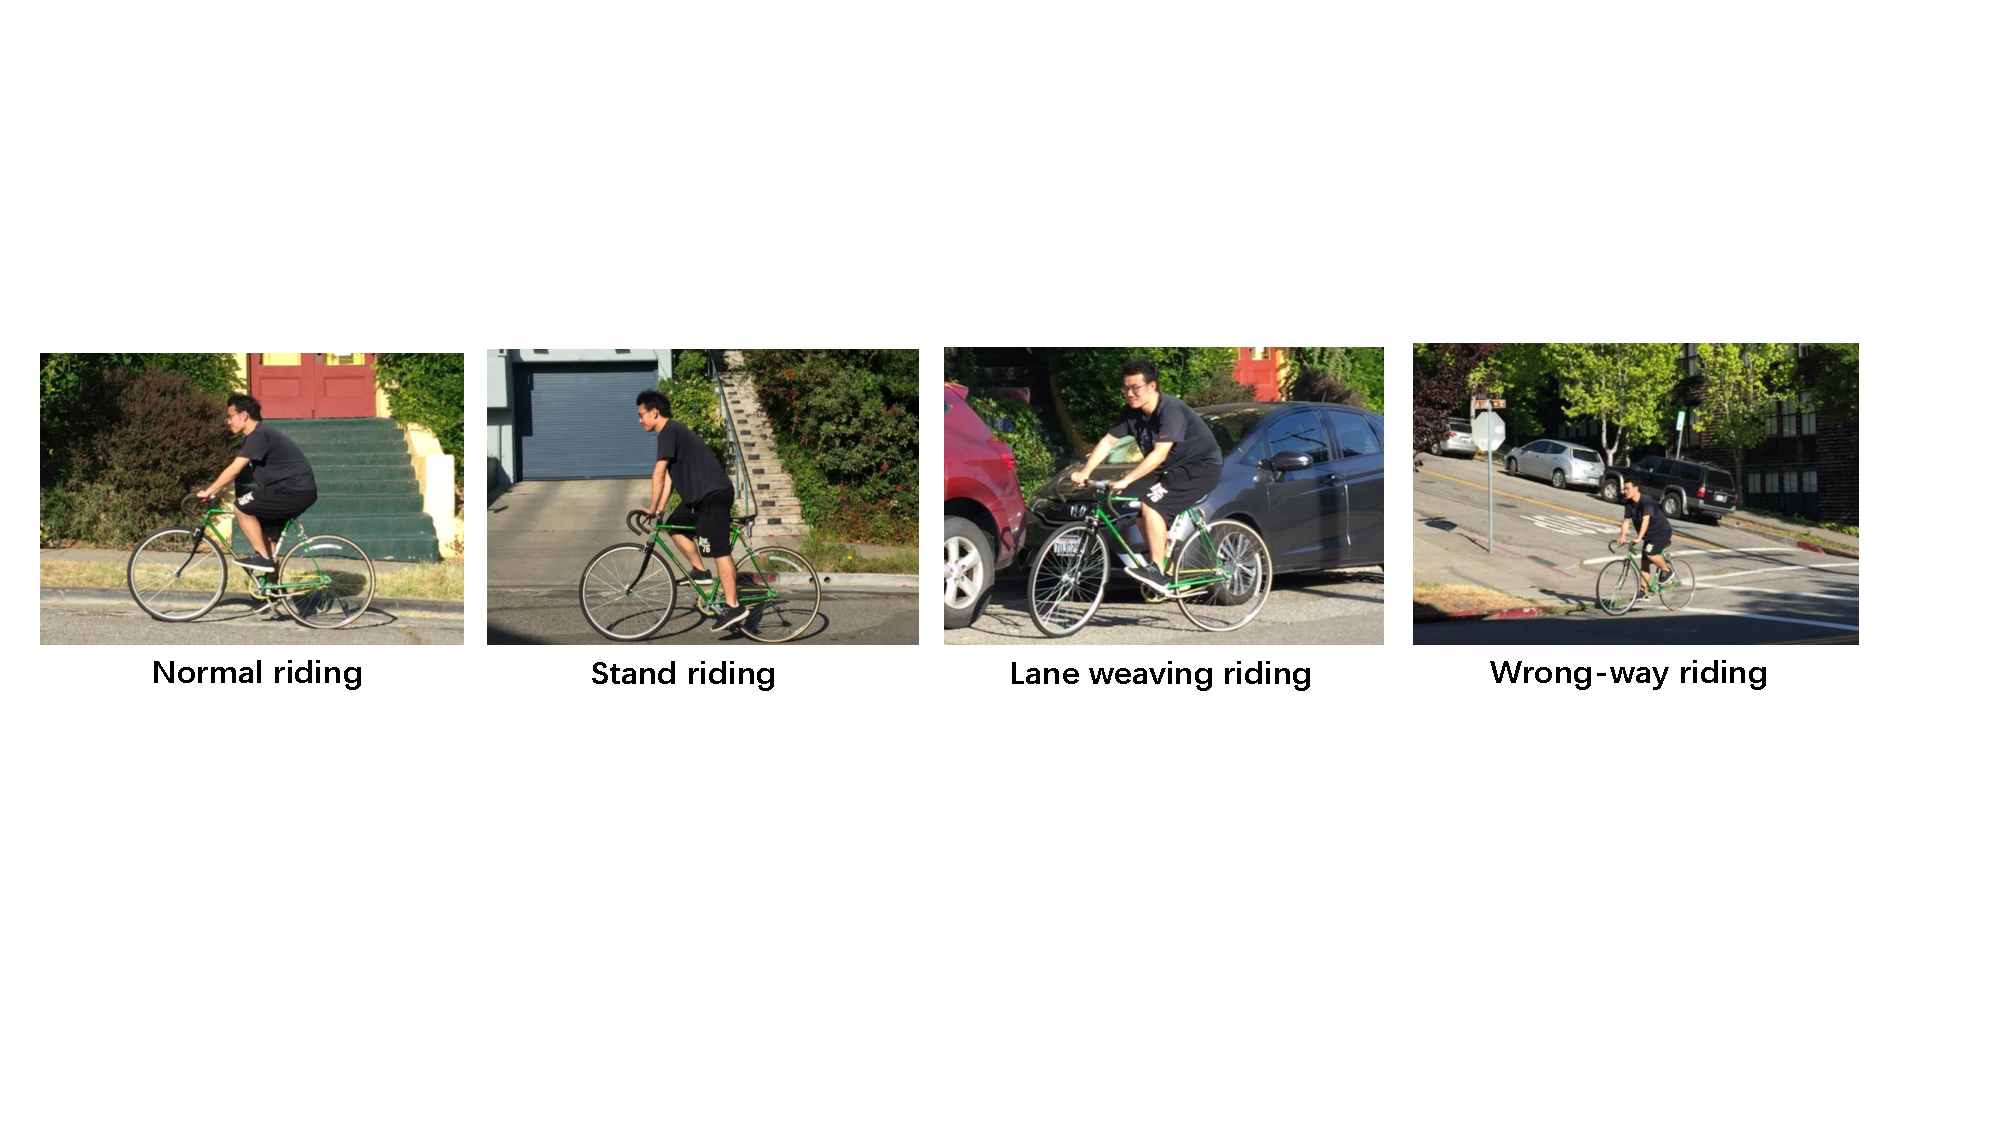
\includegraphics[width=1\columnwidth]{figures/experiment_riding.pdf}
	\caption{The GPS traces before and after noise elimination.}~\label{fig:experiment_riding}
\end{figure}
\subsection{Performance of riding event detection}
Table~\ref{confusion_matrix} shows the  prediction confusion matrix of riding movement. As shown, most of the riding movements are predicted correctly.     

\begin{table}[h]
	\centering
	\caption{The confusion matrix of riding movement}
	\label{confusion_matrix}
	\begin{tabular}{|c|c|c|c|}
		\hline
		\multirow{2}{*}{\textbf{\begin{tabular}[c]{@{}c@{}}Ground\\ Truth\end{tabular}}} & \multicolumn{3}{l|}{\textbf{Inference}}                                                                           \\ \cline{2-4} 
		& \multicolumn{1}{l|}{Normal Riding} & \multicolumn{1}{l|}{Stand Riding} & \multicolumn{1}{l|}{Lane Weaving Riding} \\ \hline
		Normal Riding                                                                    & 84.1\%                             & 7.9\%                             & 6.9\%                                    \\ \hline
		Stand Riding                                                                     & 5.6\%                              & 87.8\%                            & 4.7\%                                    \\ \hline
		Lane Weaving Riding                                                              & 10.3\%                             & 4.3\%                             & 88.4\%                                   \\ \hline
	\end{tabular}
\end{table}

\subsection{Performance of wrong-way riding direction detection}
Table~\ref{tab:wrong_way_riding} illustrates the performance of wrong-way riding direction detection. We compare the user's riding direction with the legal cycling direction of trajectories stored in the database.  
As shown, the rate of true negative are higher than 90 \%, demonstrating that \sysname can discover most wrong-way riding cases. Meanwhile, less than 15 \% false positive rate shows the legal riding behavior is rarely misclassified as the wrong-way riding.  

\begin{table}[h]
	\centering
	\caption{The performance of wrong-way riding direction detection}
	\label{tab:wrong_way_riding}
	\begin{tabular}{|c|c|c|}
		\hline
		\multirow{2}{*}{\textbf{Condition}} & \multicolumn{2}{c|}{\textbf{Test}}                            \\ \cline{2-3} 
		& \multicolumn{1}{l|}{Positive} & \multicolumn{1}{l|}{Negative} \\ \hline
		True                             & 93.2\%                        & 6.8\%                         \\ \hline
		False                              & 13.3\%                        & 86.7\%                        \\ \hline
	\end{tabular}
\end{table}

\subsection{Performance of energy consumption}
As power consumption is a practical issue in the daily operation on smartphones. We also test the energy cost of \sysname, and illustrate the results in Fig.~\ref{}.

\section{Conclusion}
Guaranteeing the bicyclist safety and keeping unexpected bike accident rate low is of great important. In this paper, we propose \sysname, a wearable and efficient mobile system to track the riding behaviors. It utilizes the embedded sensors of smartphone to monitor the dangerous riding actions and check whether the cyclist goes a wrong-side. Experimental results of 12 participants demonstrate our system is practical in daily life. 


%\marginpar{%
%  \vspace{-45pt} \fbox{%
%    \begin{minipage}{0.925\marginparwidth}
%      \textbf{Good Utilization of the Side Bar} \\
%      \vspace{1pc} \textbf{Preparation:} Do not change the margin
%      dimensions and do not flow the margin text to the
%      next page. \\
%      \vspace{1pc} \textbf{Materials:} The margin box must not intrude
%      or overflow into the header or the footer, or the gutter space
%      between the margin paragraph and the main left column. The text
%      in this text box should remain the same size as the body
%      text. Use the \texttt{{\textbackslash}vspace{}} command to set
%      the margin
%      note's position. \\
%      \vspace{1pc} \textbf{Images \& Figures:} Practically anything
%      can be put in the margin if it fits. Use the
%      \texttt{{\textbackslash}marginparwidth} constant to set the
%      width of the figure, table, minipage, or whatever you are trying
%      to fit in this skinny space.
%    \end{minipage}}\label{sec:sidebar} }


%\section{Page Size}
%All SIGCHI submissions should be US letter (8.5 $\times$ 11
%inches). US Letter is the standard option used by this \LaTeX\
%template.
%
%\section{Text Formatting}
%Please use an 8.5-point Verdana font, or other sans serifs font as
%close as possible in appearance to Verdana in which these guidelines
%have been set. Arial 9-point font is a reasonable substitute for
%Verdana as it has a similar x-height. Please use serif or
%non-proportional fonts only for special purposes, such as
%distinguishing \texttt{source code} text.
%    
%\subsubsection{Text styles}
%The \LaTeX\ template facilitates text formatting for normal (for body
%text); heading 1, heading 2, heading 3; bullet list; numbered list;
%caption; annotation (for notes in the narrow left margin); and
%references (for bibliographic entries). Additionally, here is an
%example of footnoted\footnote{Use footnotes sparingly, if at all.}
%text. As stated in the footnote, footnotes should rarely be used.
%
%\begin{figure}
%  
\includegraphics[width=0.9\columnwidth]{figures/sigchi-logo}
%  \caption{Insert a caption below each figure.}~\label{fig:sample}
%\end{figure}
%
%\subsection{Language, style, and content}
%The written and spoken language of SIGCHI is English. Spelling and
%punctuation may use any dialect of English (e.g., British, Canadian,
%US, etc.) provided this is done consistently. Hyphenation is
%optional. To ensure suitability for an international audience, please
%pay attention to the following:
%
%\begin{table}
%  \centering
%  \begin{tabular}{l r r r}
%    % \toprule
%    & & \multicolumn{2}{c}{\small{\textbf{Test Conditions}}} \\
%    \cmidrule(r){3-4}
%    {\small\textit{Name}}
%    & {\small \textit{First}}
%      & {\small \textit{Second}}
%    & {\small \textit{Final}} \\
%    \midrule
%    Marsden & 223.0 & 44 & 432,321 \\
%    Nass & 22.2 & 16 & 234,333 \\
%    Borriello & 22.9 & 11 & 93,123 \\
%    Karat & 34.9 & 2200 & 103,322 \\
%    % \bottomrule
%  \end{tabular}
%  \caption{Table captions should be placed below the table. We
%    recommend table lines be 1 point, 25\% black. Minimize use of
%    table grid lines.}~\label{tab:table1}
%\end{table}
%
%\begin{itemize}\compresslist%
%\item Write in a straightforward style. Use simple sentence
%  structure. Try to avoid long sentences and complex sentence
%  structures. Use semicolons carefully.
%\item Use common and basic vocabulary (e.g., use the word ``unusual''
%  rather than the word ``arcane'').
%\item Briefly define or explain all technical terms. The terminology
%  common to your practice/discipline may be different in other design
%  practices/disciplines.
%\item Spell out all acronyms the first time they are used in your
%  text. For example, ``World Wide Web (WWW)''.
%\item Explain local references (e.g., not everyone knows all city
%  names in a particular country).
%\item Explain ``insider'' comments. Ensure that your whole audience
%  understands any reference whose meaning you do not describe (e.g.,
%  do not assume that everyone has used a Macintosh or a particular
%  application).
%\item Explain colloquial language and puns. Understanding phrases like
%  ``red herring'' requires a cultural knowledge of English. Humor and
%  irony are difficult to translate.
%\item Use unambiguous forms for culturally localized concepts, such as
%  times, dates, currencies, and numbers (e.g., ``1-5- 97'' or
%  ``5/1/97'' may mean 5 January or 1 May, and ``seven o'clock'' may
%  mean 7:00 am or 19:00). For currencies, indicate equivalences:
%  ``Participants were paid {\fontfamily{txr}\selectfont \textwon}
%  25,000, or roughly US \$22.''
%\item Be careful with the use of gender-specific pronouns (he, she)
%  and other gender-specific words (chairman, manpower,
%  man-months). Use inclusive language (e.g., she or he, they, chair,
%  staff, staff-hours, person-years) that is gender-neutral. If
%  necessary, you may be able to use ``he'' and ``she'' in alternating
%  sentences, so that the two genders occur equally
%  often~\cite{Schwartz:1995:GBF}.
%\item If possible, use the full (extended) alphabetic character set
%  for names of persons, institutions, and places (e.g.,
%  Gr{\o}nb{\ae}k, Lafreni\'ere, S\'anchez, Nguy{\~{\^{e}}}n,
%  Universit{\"a}t, Wei{\ss}enbach, Z{\"u}llighoven, \r{A}rhus, etc.).
%  These characters are already included in most versions and variants
%  of Times, Helvetica, and Arial fonts.
%\end{itemize}
%
%% \begin{figure}
%%   \includegraphics[width=.9\columnwidth]{figures/ea-figure2}
%%   \caption{If your figure has a light background, you can set its
%%     outline to light gray, like this, to make a box around
%%     it.}\label{fig:bats}
%% \end{figure}
%
%\begin{marginfigure}[-35pc]
%  \begin{minipage}{\marginparwidth}
%    \centering
%    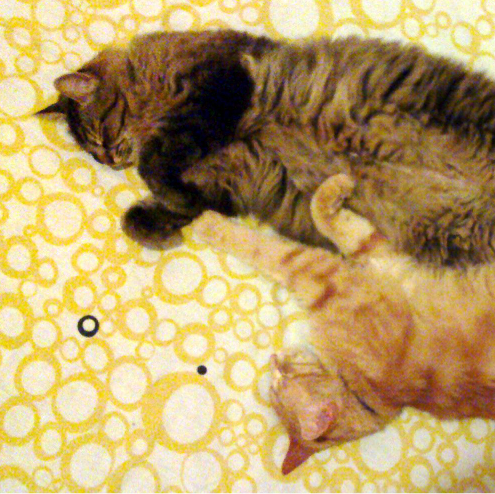
\includegraphics[width=0.9\marginparwidth]{figures/cats}
%    \caption{In this image, the cats are tessellated within a square
%      frame. Images should also have captions and be within the
%      boundaries of the sidebar on page~\pageref{sec:sidebar}. Photo:
%      \cczero~jofish on Flickr.}~\label{fig:marginfig}
%  \end{minipage}
%\end{marginfigure}
%
%\section{Figures}
%The examples on this and following pages should help you get a feel
%for how screen-shots and other figures should be placed in the
%template. Your document may use color figures (see
%Figures~\ref{fig:sample}), which are included in the page limit; the
%figures must be usable when printed in black and white. You can use
%the \texttt{\marginpar} command to insert figures in the (left) margin
%of the document (see Figure~\ref{fig:marginfig}). Finally, be sure to
%make images large enough so the important details are legible and
%clear (see Figure~\ref{fig:cats}).
%
%\section{Tables}
%You man use tables inline with the text (see Table~\ref{tab:table1})
%or within the margin as shown in Table~\ref{tab:table2}. Try to
%minimize the use of lines (especially vertical lines). \LaTeX\ will
%set the table font and captions sizes correctly; the latter must
%remain unchanged.
%
%\section{Accessibility}
%The Executive Council of SIGCHI has committed to making SIGCHI
%conferences more inclusive for researchers, practitioners, and
%educators with disabilities. As a part of this goal, the all authors
%are asked to work on improving the accessibility of their
%submissions. Specifically, we encourage authors to carry out the
%following five steps:
%\begin{itemize}\compresslist%
%\item Add alternative text to all figures
%\item Mark table headings
%\item Generate a tagged PDF
%\item Verify the default language
%\item Set the tab order to ``Use Document Structure''
%\end{itemize}
%
%For links to instructions and resources, please see:
%\url{http://chi2016.acm.org/accessibility}
%
%Unfortunately good tools do not yet exist to create tagged PDF files
%from Latex. \LaTeX\ users will need to carry out all of the above
%steps in the PDF directly using Adobe Acrobat, after the PDF has been
%generated.
%
%For more information and links to instructions and resources, please
%see:
%\url{http://chi2016.acm.org/accessibility}.
%
%\begin{figure*}
%  \centering
%  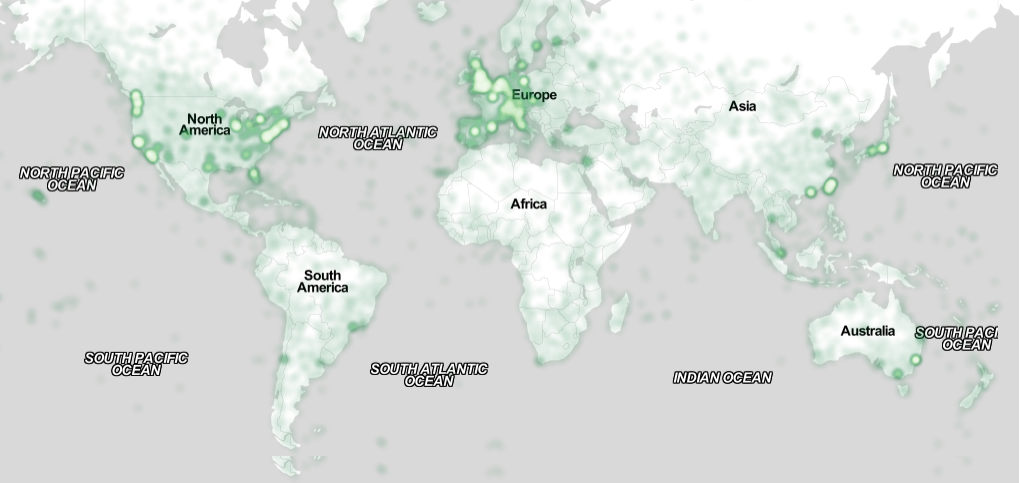
\includegraphics[width=1.3\columnwidth]{figures/map}
%  \caption{In this image, the map maximizes use of space. You can make
%    figures as wide as you need, up to a maximum of the full width of
%    both columns. Note that \LaTeX\ tends to render large figures on a
%    dedicated page. Image: \ccbynd~ayman on Flickr.}~\label{fig:cats}
%\end{figure*}
%
%\section{Producing and Testing PDF Files}
%We recommend that you produce a PDF version of your submission well
%before the final deadline. Your PDF file must be ACM DL Compliant and
%meet stated requirements,
%\url{http://www.sheridanprinting.com/sigchi/ACM-SIG-distilling-settings.htm}.
%
%\marginpar{\vspace{-23pc}So long as you don't type outside the right
%  margin or bleed into the gutter, it's okay to put annotations over
%  here on the left, too; this annotation is near Hawaii. You'll have
%  to manually align the margin paragraphs to your \LaTeX\ floats using
%  the \texttt{{\textbackslash}vspace{}} command.}
%
%\begin{margintable}[1pc]
%  \begin{minipage}{\marginparwidth}
%    \centering
%    \begin{tabular}{r l}
%       {\small \textbf{First}}
%      & {\small \textbf{Location}} \\
%      \toprule
%       22.5 & Melbourne \\
%       22.0 & Bogot\'a \\
%      \bottomrule
%    \end{tabular}
%    \caption{A simple narrow table in the left margin
%      space.}~\label{tab:table2}
%  \end{minipage}
%\end{margintable}
%Test your PDF file by viewing or printing it with the same software we
%will use when we receive it, Adobe Acrobat Reader Version 10. This is
%widely available at no cost. Note that most
%reviewers will use a North American/European version of Acrobat
%reader, so please check your PDF accordingly.
%
%\section{Acknowledgements}
%We thank all the volunteers, publications support, staff, and authors
%who wrote and provided helpful comments on previous versions of this
%document. As well authors 1, 2, and 3 gratefully acknowledge the grant
%from NSF (\#1234--2222--ABC). Author 4 for example may want to
%acknowledge a supervisor/manager from their original employer. This
%whole paragraph is just for example. Some of the references cited in
%this paper are included for illustrative purposes only.
%
%\section{References Format}
%Your references should be published materials accessible to the
%public. Internal technical reports may be cited only if they are
%easily accessible and may be obtained by any reader for a nominal
%fee. Proprietary information may not be cited. Private communications
%should be acknowledged in the main text, not referenced (e.g.,
%[Golovchinsky, personal communication]). References must be the same
%font size as other body text. References should be in alphabetical
%order by last name of first author. Use a numbered list of references
%at the end of the article, ordered alphabetically by last name of
%first author, and referenced by numbers in brackets. For papers from
%conference proceedings, include the title of the paper and the name of
%the conference. Do not include the location of the conference or the
%exact date; do include the page numbers if available.
%
%References should be in ACM citation format:
%\url{http://www.acm.org/publications/submissions/latex_style}.  This
%includes citations to Internet
%resources~\cite{CHINOSAUR:venue,cavender:writing,psy:gangnam}
%according to ACM format, although it is often appropriate to include
%URLs directly in the text, as above. Example reference formatting for
%individual journal articles~\cite{ethics}, articles in conference
%proceedings~\cite{Klemmer:2002:WSC:503376.503378},
%books~\cite{Schwartz:1995:GBF}, theses~\cite{sutherland:sketchpad},
%book chapters~\cite{winner:politics}, an entire journal
%issue~\cite{kaye:puc},
%websites~\cite{acm_categories,cavender:writing},
%tweets~\cite{CHINOSAUR:venue}, patents~\cite{heilig:sensorama},
%games~\cite{supermetroid:snes}, and
%online videos~\cite{psy:gangnam} is given here.  See the examples of
%citations at the end of this document and in the accompanying
%\texttt{BibTeX} document. This formatting is a edited version of the
%format automatically generated by the ACM Digital Library
%(\url{http://dl.acm.org}) as ``ACM Ref''. DOI and/or URL links are
%optional but encouraged as are full first names. Note that the
%Hyperlink style used throughout this document uses blue links;
%however, URLs in the references section may optionally appear in
%black.
%
%\balance{}
%
\bibliographystyle{SIGCHI-Reference-Format}
\bibliography{sample}
\end{document}

%%% Local Variables:
%%% mode: latex
%%% TeX-master: t
%%% End:
